\chapter{Fundamentação}\label{chp:LABEL_CHP_2}

Esse capitulo trata da mineração de dados descrevendo os principais objetivos desse campo de estudos, suas principais técnicas e aplicabilidades. Ele também descreve a técnica de \textit{Web Scraping}.

\section{Mineração dos Dados}

% Estrutura:
% Intro a mineração de dados. Motivação e "nascimento"
% Processo de descoberta de conhecimento
% Pequena introdução ao CRISP.
% Preparação de dados
% As técnicas da mineração de dados
% Os tipos de método da mineração de dados
% Exemplo de algoritmo relacionando com uma técninca e um tipo de método
% Chamar atenção para que pesquisadores criam dados para estudar por não ter acesso a eles.
% Estabelecer que uma das limitações é o formato de entrada
% Introduzir a mineração de texto
% Introduzir mineração de mídias sociais
% Introduzir mineração de dados. Definição, problema que motiva.

Tradicionalmente, para extrair conhecimento de dados, é necessária uma análise e interpretação manual dos mesmos \cite{fayyad1996data}. \citeonline{fayyad1996data} exemplificam dizendo que é comum que, na área de saúde, sejam gerados relatórios periódicos feitos por especialistas por meio da análise dos dados do plano de saúde e que, com base nesses relatórios, são feitos os planejamentos gerenciais e futuras tomadas de decisão.

Porém, com o volume de dados crescendo drasticamente, esse método de análise está se tornando impraticável para muitos domínios. Mesmo quando é possível realizar a análise, esse processo pode ser lento, caro e muito subjetivo \cite{fayyad1996data}. Empresas gastam milhões de reais para coletar e armazenar dados sem que informações uteis possam ser identificadas \cite{camilo2009mineraccao}. Foi com o intuito de solucionar esse problema que, no final da década de 80, foi proposta a Mineração de Dados \cite{camilo2009mineraccao}.

Alguns autores tratam a Descoberta de Conhecimento nas Bases de Dados (\textit{Knowledge Discovery in Databases} - KDD) como sinônimo de Mineração de dados, enquanto outros tratam a Mineração de Dados como uma parte do processo de KDD \cite{camilo2009mineraccao}. Para \citeonline[p.~40-41, tradução nossa]{fayyad1996data}, KDD é "um processo não trivial de identificação de novos padrões válidos, úteis e compreensíveis". \citeonline{cortes2002mineraccao} definem Mineração de Dados como:

\begin{quote}
    (...) um processo altamente cooperativo entre homens e máquinas, que visa a exploração de grandes bancos de dados, com o objetivo de extrair conhecimentos através do reconhecimento de padrões e relacionamento entre variáveis, conhecimentos esses que possam ser obtidos por técnicas comprovadamente confiáveis e validados pela sua expressividade estatística \cite[p.~1-2]{cortes2002mineraccao}.
\end{quote}

O processo de mineração é iterativo, interativo e dividido em fases \cite{camilo2009mineraccao}. \citeonline{fayyad1996data} separa o processo de \textit{KDD} em seleção, pré-processamento, transformação, mineração de dados e interpretação/avaliação, ilustrado na figura \ref{fig:kdd-geral}.

\begin{figure}[h!]
    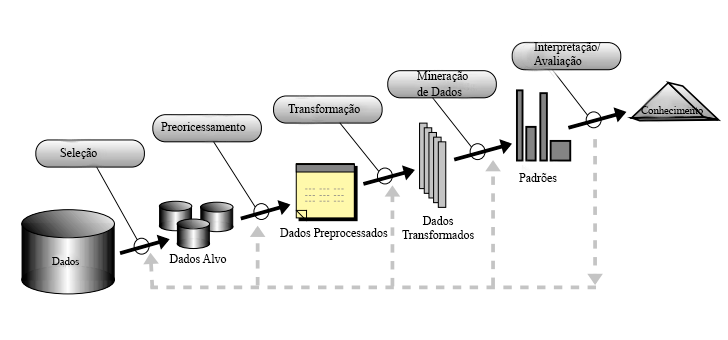
\includegraphics[width=\textwidth]{img/kdd.png}
    \caption{Uma visão geral dos passos que compõem um processo KDD. Adaptado de \citeonline{fayyad1996data}}
    \centering
    \label{fig:kdd-geral}
\end{figure}

O processo CRISP-DM (\textit{Cross-Industry Standard Processo of Data Mining}), que pode ser considerado o de maior aceitação hoje em dia \cite{camilo2009mineraccao}, é dividido em seis fases, apresentadas na figura \ref{fig:crisp}: entendimento do negócio, entendimento dos dados, preparação dos dados, modelagem, avaliação e implantação \cite{olson2008advanced}.

\begin{figure}[h]
\centering
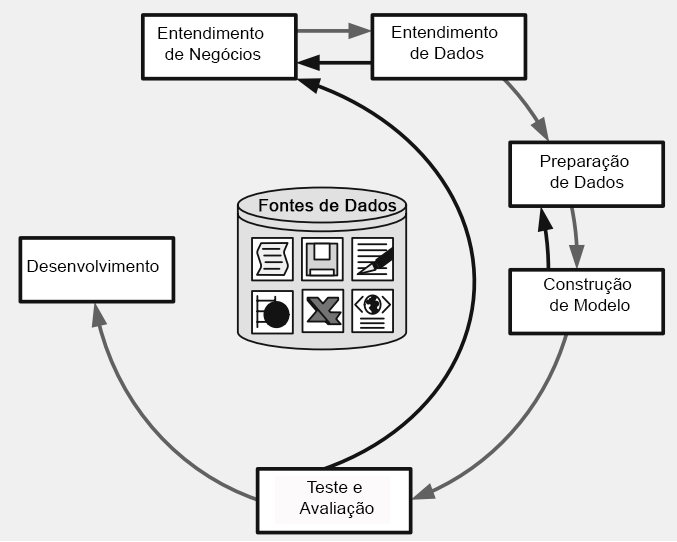
\includegraphics[width=0.8\textwidth]{img/crisp.png}
\caption{Processo CRISP-DM. Adaptado de \citeonline{olson2008advanced}}
\label{fig:crisp}
\end{figure}


Os dados podem ser qualitativos ou quantitativos. O primeiro são dados com valores nominais e categóricos. Já o segundo, diz respeito a dados com valores numérico, sejam eles discretos ou contínuos \cite{camilo2009mineraccao}. Para escolher o método a ser utilizado, é fundamental entender qual o tipo do dados será utilizado como entrada, e para utilizá-los, geralmente é preciso prepará-los \cite{camilo2009mineraccao}. \citeonline{camilo2009mineraccao} ressaltam:

\begin{quote}
    Devido às diversas origens possíveis, é comum que os dados não estejam preparados para que os métodos de Mineração de Dados sejam aplicados diretamente. Dependendo da qualidade desses dados, algumas ações podem ser necessárias. Este processo de limpeza dos dados geralmente envolve filtrar, combinar e preencher valores vazios
    \cite[p.~4]{camilo2009mineraccao}.
\end{quote}

A fase de preparação dos dados pode ocupar, sozinha, a maior parte do processo \cite{camilo2009mineraccao}. Para melhor entender os dados de forma a auxiliar na escolha de como prepará-los, são utilizados diversas técnicas de visualização de dados \cite{camilo2009mineraccao}. Após obtido conhecimento sobre dados, é possível escolher a melhor forma de prepará-lo para a mineração. Na preparação se realiza a limpeza de dados, integração de dados, transformação dos dados e redução dos dados \cite{han2011data}.

Muita vezes, quando se cria um modelo para um conjunto de dados de um problema, ele não se mostra satisfatório para um outro conjunto de dados do mesmo problema. Isso se dá pois o modelo se torna enviesado aos dados com os quais ele foi treinado. Esse efeito é conhecido como efeito \textit{Bias}. Para evitar isso, normalmente se divide o conjunto em três partes: conjunto de treinamento, conjunto de testes e conjunto de validação \cite{camilo2009mineraccao}.

\citeonline{camilo2009mineraccao} ressaltam que, apesar da existência massiva de dados sob posse das empresas, normalmente esses dados não são disponibilizados para pesquisadores. Devido a isso é comum se criar algoritmos teóricos e validá-los com dados sintéticos. Desta forma, não tendo a possibilidade de testá-los em um ambiente real.

A mineração de dados possui dois principais objetivos: predição e classificação. A predição consiste em usar parte dos dados ou dos campos para inferir valores de outros campos ou valores futuros dos mesmos. A classificação foca em encontrar padrões descritivos que humanos possam interpretar \cite{fayyad1996data}. 

Existem diversas técnicas para auxiliar a alcançar os objetivos. Dentre elas estão: classificação, regressão, descrição, agrupamento, associação e predição \cite{fayyad1996data}. Cada uma dessas técnicas possuem diversos métodos e algoritmos, que podem ser supervisionados, não-supervisionados ou uma variação entre os dois \cite{camilo2009mineraccao}.

Regressão Linear, por exemplo, é um método supervisionado de predição, que objetiva encontrar um possível valor futuro para uma variável. O método consiste em encontrar uma função linear a partir dos dados existentes onde o valor de \textit{y} é estimado em função de uma variável \textit{x} \cite{camilo2009mineraccao}.

\begin{figure}[h]
\centering
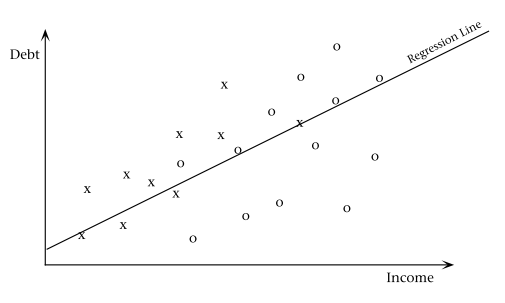
\includegraphics[width=0.8\textwidth]{img/linear-reg.png}
\caption{Uma regressão linear simples de um conjunto de dados de empréstimo. Adaptado de \citeonline{fayyad1996data}}
\label{fig:linear-reg}
\end{figure}

Uma das limitações da mineração de dados está no formato do dado de entrada. Inicialmente pensadas para serem aplicadas em dados estruturados em bancos de dados ou arquivos, as técnicas de mineração podem não ter mesma eficácia ao lidar com dados em outros formatos, \textit{e.g.} multimídia, texto, espacial. Devido a isso muitos estudos tratando a mineração de dados complexos vem sendo feitos \cite{camilo2009mineraccao}. Um exemplo disso é a mineração de textos.

Devido à falta de estrutura, dados textuais normalmente são manipulados por meio de motores de busca, diferente de dados estruturados, que normalmente são manipulados por meio de sistemas de banco de dados. Motores de busca são eficientes no objetivo de levar o usuário à informação correta no tempo correto, mas a mineração de texto é mais que isso. Mineração de texto pode ajudar o usuário a digerir a informação e ajudar na tomada de decisão \cite{aggarwal2012mining}. \citeonline{aggarwal2012mining} completam:

\begin{quote}
    Existem diversas aplicações para a mineração de texto onde o objetivo primário é analisar e descobrir algum padrão interessante, incluindo tendencias e \textit{outliers}, em dados textuais, e a noção de busca não é essencial ou mesmo relevante \cite[p.~2, tradução nossa]{aggarwal2012mining}.
    % Text mining can be regarded as go- ing beyond information access to further help users analyze and digest information and facilitate decision making.There are also many applica- tions of text mining where the primary goal is to analyze and discover any interesting pattterns, including trends and outliers, in text data, and the notion of a query is not essential or even relevant.
\end{quote}

\citeonline{marfianto2018whatsapp} apresentam o que pode ser usado com um exemplo de uso de mineração de texto. O trabalho utiliza de técnicas de mineração de texto para fazer uma análise forense das mensagens do WhatsApp de um suspeito com o intuito de ajudar a extrair evidências criminalísticas.

% [
% \textbf{Preciso de um jeito de fazer uma ponte entre mineração de texto e mineração de opinião e mineração de redes sociais.
% Essa ponte é feita no livro \cite{aggarwal2012mining}, mas não consigui pensar num jeito de fazer de forma enxuta e rápida.}
% ]

Uma das fontes de texto mais comuns são as redes sociais. Elas permitem que as pessoas se expressem de forma rápida e livre em contextos muito abrangentes. Para minerar texto dessas fontes é necessário técnicas específicas, pois podem conter um vocabulário coloquial e sem padronização. Métodos que fazem uso tanto das conexões da rede social quanto do conteúdo, por exemplo, conseguem prover resultados mais eficientes que os que usam apenas o conteúdo ou conexões \cite{aggarwal2012mining}. 

As formas mais comuns de mineração de conteúdo da internet é feito através de mineração de dados não-estruturados, mineração de dados estruturados, mineração de dados semi-estruturados ou mineração de dados multimídia. A coleta de dados para mineração é uma tarefa importante para a mineração de dados não-estruturados e um dos maiores desafios, devido à complexidade de todas as \textit{tags} \textit{HTML} que podem estar presentes. \textit{Web Scrapers} ajudam a simplificar essa tarefa \cite{dastidar2016intelligent}.

% The major forms of web content mining are done in the following ways:
% ? Unstructured data mining ? Structured data mining ? Semi-structured data mining

% Under the subtopic of unstructured data mining comes the mining of web documents which this paper deals with. Personal Information retrieval is a challenging task when it comes to mining from web pages, primarily because of the complexity of all the HTML tags that may be present. Web scrapers help a great deal in simplifying the task.


% Exemplificar mineração de dados com os diferentes tipos

\section{\textit{Web Scraping}}

A internet se tornou a maior fonte de dados do mundo \cite{banerjee2014website}. A geração de dados e o crescimento de sua taxa está aumentando a cada dia \cite{dastidar2016intelligent}. A internet foi projetada para que seja fácil para que pessoas encontrem informações \cite{banerjee2014website}. Usuários na internet podem usufruir abundantemente de serviços e informação, \textit{e.g.} comércio eletrônico, \textit{websites}, jornais eletrônicos, redes sociais e blog \cite{dastidar2016intelligent}. Mas, se a única forma de acessar esses dados for por meio de um navegador \textit{web}, uma grande variedade de possibilidades será perdida \cite{mitchell2018web}. 

Muitas empresas, com o objetivo de localizar, capturar e guardar um enorme volume de informação que precisam de \textit{websites}, ainda usam de métodos tradicionais de extração de dados da internet, como o manual "copia e cola" \cite{banerjee2014website}. O processo de extração manual consiste na empresa contratar uma grande quantidade de funcionários e orientá-los a fazer a extração navegando pelas páginas copiando os dados para um banco de dados \cite{banerjee2014website}. Tal processo, além de muito caro, também é muito suscetível a erros humanos \cite{banerjee2014website}. 

Outra possibilidade para recuperar essas informações seria por meio das APIs (\textit{Application Program Interface}). Uma \textit{API} define uma sintaxe padronizada que permite uma parte de um software se comunicar com uma outra parte, mesmo que eles tenham sido escritos em linguagens diferentes ou estruturados de forma diferente \cite{mitchell2018web}. É possível encontrar \textit{APIs} de diversos tipos de dados que podem ser utilizados, \textit{e.g}. postagens do \textit{Twitter}\footnote{www.twitter.com}, paginas do \textit{Wikipedia}\footnote{www.wikipedia.com}. Apesar de ser preferível fazer uso das APIs, elas podem não existir para o dado desejado ou possuir limitações de acesso, \textit{e.g} quantidade de acessos por dia \cite{mitchell2018web}.

Páginas HTML é a principal ferramenta de formação de informação na internet. \citeonline[p.~25]{dastidar2016intelligent} define \textit{Web Scraping} como o processo de extrair informações úteis dessas paginas usando qualquer linguagem de programação. Para \citeonline{mitchell2018web}, é na prática uma vasta variedade de técnicas de programação e tecnologias, como análise de dados, análise de linguagem natural e segurança da informação. \citeonline{mitchell2018web} ainda define teoricamente como:

\begin{quote}
    (...) a prática de recuperar dados por meio de qualquer outro meio que não um programa interagindo com uma API (ou, obviamente, por meio de um humano usando um navegador). Normalmente, isso é alcançado escrevendo um programa automatizado que consulta um servidor \textit{web}, requisita dados (normalmente em forma de HTML e outros arquivos que compõem uma página \textit{web}), e então analisa esses dados pra extrair a informação necessária
    \cite[p.~ix, tradução nossa]{mitchell2018web}.
    % is the practice of gathering data through any means other than a program interacting with an API (or, obviously, through a human using a web browser). This is most commonly accomplished by writing an automated program that queries a web server, requests data (usually in the form of HTML and other files that compose web pages), and then parses that data to extract needed information.
\end{quote}

Uma das aplicabilidades da técnica de \textit{Web Scraping} é na mineração de dados na internet \cite{dastidar2016intelligent}. Mineração de internet, como explica \citeonline[p.~197-198, tradução nossa]{shi2009web}, "é uma área de pesquisa que tenta identificar pedaços de informação aplicando técnicas de mineração de dados e aprendizado de máquina a documentos e dados da internet". As principais formas de mineração de conteúdo na internet é feito por meio de mineração de dados não-estruturados, mineração de dados estruturados, mineração de dados semi-estruturados e mineração de dados multimídia \cite{dastidar2016intelligent}.

Devido à complexidade das \textit{tags} \textit{HTML}, recuperar informações de documentos na internet pode se tornar uma tarefa complicada, mesmo sendo uma parte importante da mineração de dados não-estruturados. \textit{Web Scraping} simplifica significativamente essa tarefa \cite{dastidar2016intelligent}.

Um exemplo de uso de \textit{Web Scrapping} pode ser encontrado no trabalho de \citeonline{boeing2017new}. Os autores extraíram a listagem de aluguéis de casas nos Estados Unidos do site \textit{Craiglist}\footnote{http://craigslist.org/} e conseguiram demonstrar novas informações sobre padrões de distribuição espacial do mercado de casas no país de forma mais rica que utilizando outras fontes de informações públicas, como o censo.